\chapter{Projekt rękawicy}
\label{ch:rekawica}
Istotą poniższego rozdziału jest pokazanie użytych w projekcie podzespołów i technologii oraz lepsze zrozumienie powodów dla których to właśnie te produkty zostały wybrane. Po zapoznaniu się z motywem, zostanie szczegółowo opisana specyfikacja tych produktów a także sposób ich poskładania w spójną całość, co sprawiło pewne problemy względem oryginalnego szkicu - próby oraz efekty rozwiązywania tych problemów również zostaną opisane w tym rozdziale. Po nakreśleniu podstawowych założeń projektu zostanie zaprezentowana finałowa wersja, a także szczegółowo zostanie omówiony kod rękawicy-kontrolera, który jest obsługiwany przez mikrokontroler i stanowi najważniejszą część tego projektu.  Po zaznajomieniu się z kodem aplikacji, będą zaprezentowane wady oraz możliwe ulepszenia projektu, jakie ukazały się w trakcie prac nad aplikacją obsługującą i wykorzystującą dane z rękawicy, w celu ich prezentacji o czym będzie więcej mowa w rozdziale~\ref{ch:aplikacja} dotyczącym tejże właśnie aplikacji.
\improvement{Następny rozdział? - Dodaj sekcje mówiącym o wybraniu arduino ide oraz nie wybraniu istniejacych sdk aby napisac wlasne polaczenie BLE w javie bez unity}

\section{Przegląd podzespołów i technologii użytej w projekcie}
\label{sec:przeglad}
Jak dowiedzieliśmy się z rozdziału \ref{ch:komponenty} dotyczącego podstawowych komponentów rękawic, kluczowym dla powodzenia projektu jest ustalenie \begin{itemize}
\item orientacji
\item położenia 
\item pozycji palców
\end{itemize} W tym celu należy zebrać informacje z czujników, a następnie wszystkie te informacje należy przesłać do pożądanego urządzenia. Elementem które pozwala to osiągnąć w tym projekcie jest mikrokontroler Arduino nano 33 BLE, który odpowiada za dostarczenie informacji z żyroskopu, akcelerometru a także czujników wygięcia. Zasady działania pierwszych dwóch zostały opisane z podrozdziałach~\ref{subsec:gyro} oraz ~\ref{subsec:acc}. Natomiast w poniższych podrozdziałach zostanie opisane rozwiązanie zastosowane do odczytu położenia palców, zasada działania przy wykorzystaniu rezystorów oraz sposób połączenia wszystkich wspomnianych elementów w jeden finałowy kontroler.
	
	
	\subsection{Mikrokontroler}
	\label{subsec:arduino}
	Jak przed chwilą wspomniano, w projekcie wykorzystywana jest płytka od Arduino, która nosi nazwę Nano 33 BLE. Jest to małych rozmiarów płytka o  wymiarach 45 x 18 mm, pozwalająca na wysoką wydajność przy jednoczesnym małym poborze prądu, co zapewnia użyty mikrokontroler nRF52480 o taktowaniu 64 MHz. Do dyspozycji mamy również pamięć RAM o pojemności 256 kB oraz pamięć Flash o pojemności 1 MB. Warto na wstępie zauważyć że Nano 33 BLE pracuje domyślnie wyłącznie z napięciem 3,3 V. Nie należy podłączać bezpośrednio zasilania o większym napięciu. W celu podłączenia zasilania 5 V należy zlutować zworkę znajdującą się pomiędzy pinami RDT oraz A7 - temat ten nie zostaje jednak poruszony w tej pracy, ponieważ na potrzeby projektu używane jest zasilanie poprzez złącze micro USB które to również jest obsługiwane. Płytka ta posiada wiele użytecznych sensorów, jednak na potrzeby tej pracy została wybrana z powodu wbudowanej inercyjnej jednostki pomiarowej, dzięki czemu można było uprościć konstrukcję   oraz zmniejszyć ilość połączeń na rękawicy, wbudowanego modułu Bluetooth - a w tym przypadku modułu Bluetooth Low Energy obsługiwanego w standardzie 5.0, a to wszystko w przystępnej cenie co również było jednym z kryteriów przy tworzeniu tego projektu. Płytkę w momencie tworzenia tej pracy można kupić za 119 zł. Wartym uwagi jest fakt możliwości zakupu płytki bez wyprowadzonych złącz, co w przypadku opisywanego projektu pozwoli na zmniejszenie wymiarów oraz większą swobodę montażu.~\cite{botland-arduino}
	
	Z najważniejszych elementów układu płytki należy wiedzieć że posiada ona dwie diody po dwóch stronach portu micro USB - zielona indykuje podłączone zasilanie, natomiast pomarańczowa zaczyna mrugać gdy jest przesyłany kod do mikrokontrolera. Oprócz tego do dyspozycji są dwa piny wyjściowe zasilające o napięciu 3,3 V oraz 5 V, jeden pin zasilający wejściowy, którego ograniczenia zostały wspomniane w poprzednim paragrafie, a także dwa piny uziemiające, po jednym z każdej strony płytki. Posiada ona piny zarówno analogowe jak i cyfrowe, jednak na potrzeby tego projektu zostały użyte jedynie piny analogowe, których do dyspozycji jest aż osiem umiejscowionych po jednej stronie, przy czym warto zwrócić uwagę że piny A4 oraz A5 używane są jako magistrala I2C w związku z czym zalecane jest nie stosowanie tych wejść analogowych. Szczegółowy opis wejść/wyjść płytki przedstawiony jest na grafice~\ref{fig:arduino}.
	
\begin{figure}[h]
\centering
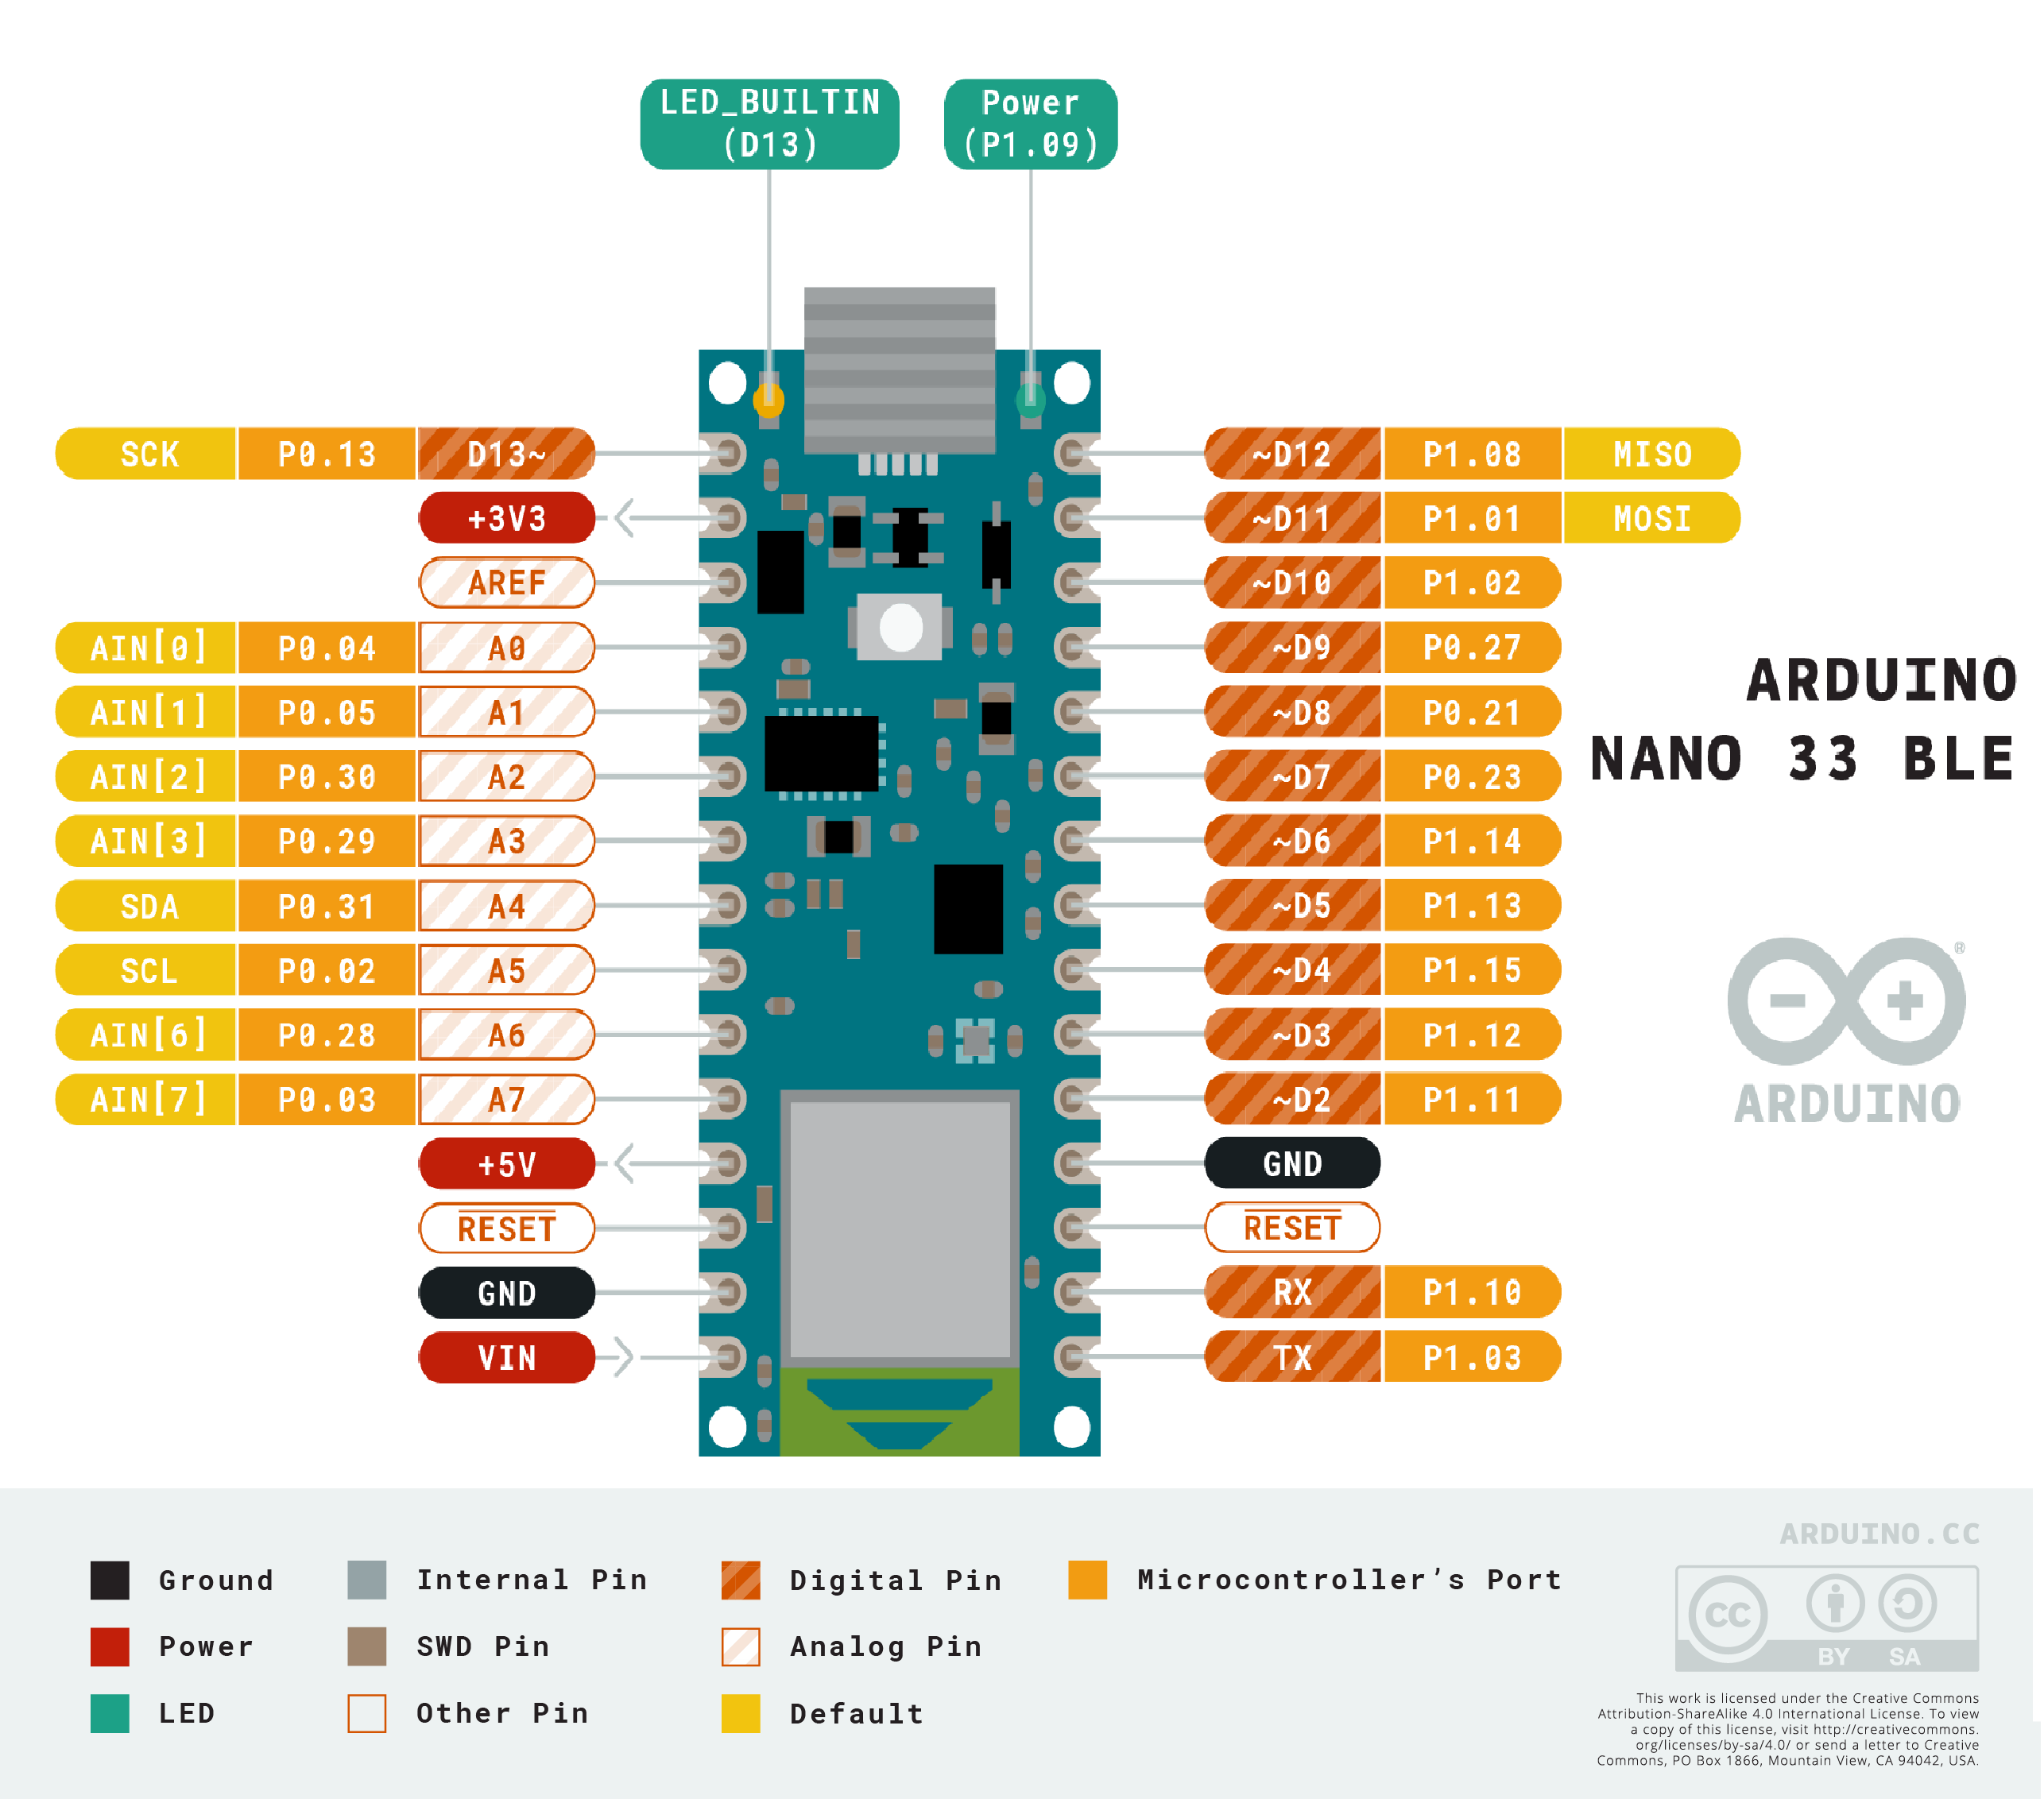
\includegraphics[scale=0.65]{arduino}
\caption{Opis wejść oraz wyjść Arduino Nano 33 BLE z podręcznika producenta.}
\label{fig:arduino}
\end{figure}

	W tym projekcie wykorzystano zasilanie poprzez złącze micro USB, wyjście o napięciu 3,3 V w celu uzyskania odczytów z czujników wygięcia na pinach analogowych A0, A1, A3, A6 oraz A7, o których zostanie więcej powiedziane w punkcie~\ref{sec:budowa}, a także uziemienie znajdujące się po tej samej stronie płytki.

	\subsection{Czujnik wygięcia}
	\label{subsec:wygiecie}	
	Kluczowym dla działania kontrolera jest możliwość określenia pozycji palców względem dłoni. Ma to wiele zastosowań zarówno wizualnych jak i praktycznych. Ważne jest aby odwzorować świat rzeczywisty tak dokładnie jak to możliwe - im lepsze odwzorowanie tym bardziej zmysły użytkownika zostaną oszukane, podwyższając komfort użytkowania technologii wirtualnej rzeczywistości. Za stroną praktyczną natomiast przemawia możliwość śledzenia palców w celu dokładnego ich użycia w stworzonym środowisku np. do ściskania i podnoszenia obiektów czy też korzystania z klawiatury wirtualnej. Jak wspomniano w rozdziale~\ref{ch:komponenty} dotyczącym komponentów komercyjnych rękawic - większość producentów decyduję się na użycie wielu inercyjnych jednostek pomiarowych, na podstawie których są w stanie dokładnie określić położenia każdej części palca, bądź też specjalistycznych sensorów służących do pomiaru stopnia wygięcia czujnika względem pozycji prostej. \improvement{Dodaj jakieś źródło flex sensor albo imu na palcach}
Czujnik ten po podłączeniu do prądu zwiększa swój opór wraz ze zwiększonym stopniem odchylenia. Oba te rozwiązania pomimo wysokiej dokładności pomiarów nie są rozwiązaniami tanimi. W związku z tym na potrzeby stworzenia taniego kontrolera, należało znaleźć rozwiązanie bardziej przystępna a jednocześnie pozwalające na osiągnięcie tego samego celu.
	
	Aby osiągnąć postawione założenia zostały skonstruowane czujniki wygięcia w domowych warunkach. Rozwiązanie to jest często używane do osiągnięcia pomiaru stopnia wygięcia bez konieczności wydawania ponad 100 zł na jeden czujnik~\cite{flex-sensor}. Jest ono stosunkowo proste w założeniach i wymaga jedynie dwóch kluczowych elementów. Tkaniny przewodzącej o specjalnych właściwościach oraz dwóch przewodników po obu stronach materiału. Z jednej strony zostanie podłączone napięcie z drugiej natomiast uziemienie. Ważnym jest aby połączenia te się ze sobą nie stykały w żadnym punkcie a jedynie zostały nałożone na siebie, z tkaniną ściśniętą pomiędzy nimi - dzięki temu mamy pewność że odczyty które otrzymamy będą prawidłowe. Pozostaje odpowiedzieć na pytanie jakiego rodzaju materiał należy wykorzystać. Na rynku znajdziemy wiele rodzajów materiałów które zmieniają swój opór w zależności od spełnienia takich kryteriów jak nacisk, temperatura, rozciągnięcie czy też właśnie zgięcie materiału. Pomimo próby uzyskania materiału który zmienia swój opór w zależności od rozciągnięcia, co pozwoliłoby na skonstruowanie części na palce rękawiczki z tego materiału, zapewniając dokładniejszy i bardziej estetyczny efekt końcowy, w momencie projektowania rękawicy był on jedynie możliwy do sprowadzenia ze stanów, co nie było najtańszym rozwiązaniem. W związku z tym zdecydowano się na użycie foli Velostat która jest czuła na nacisk or zginanie~\cite{velostat}. W roli przewodnika wybrano nić przewodzącą, która zapewniła potrzebną elastyczność oraz możliwość przymocowania poszczególnych elementów przy jednoczesnym zapewnieniu funkcjonalności. Elementy te zostały sklejone na kawałku taśmy samoprzylepnej oraz dodatkowo sklejone przy brzegu aby nić nie wyśliznęła się w trakcie korzystania z czujnika. Efekt końcowy jest widoczny na zdjęciu~\ref{fig:sensor}. W celu otrzymania pomiarów wszystkich palców zostało wykonanych pięć takich sensorów, o szerokości 15 mm; dwa o długości 8 cm, dwa o długości 10 cm a także jeden 11 cm, w celu jak najlepszego dopasowania względem miejsca na palce na zakupionej rękawicy do której sensory zostaną przymocowane, co można zobaczyć na zdjęciu~\ref{fig:glove}.
	
\begin{figure}[h]
\centering
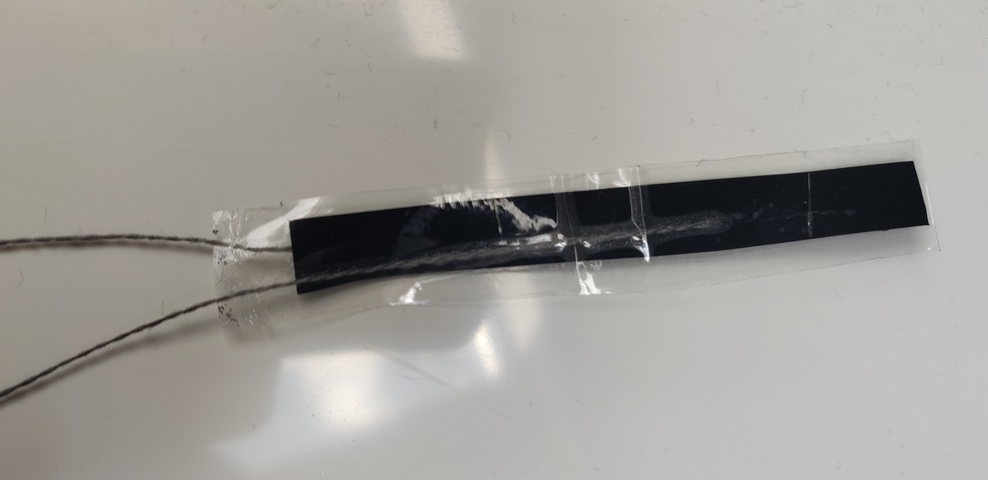
\includegraphics[scale=0.65,width=\textwidth]{flex-sensor}
\caption{Sensor wygięcia własnego wykonania}
\label{fig:sensor}
\end{figure}	

	\subsection{Rezystor}
	\label{subsec:rezystor}	
	Rezystor, potocznie zwany opornikiem, jest to prosty element elektroniczny, posiadający jedynie wyjścia z dwóch stron elementu łączącego. Element ten tworzy opór, powodując ograniczenie przepływającego przez niego prądu gdy jest włączony do obwodu szeregowo. Opór ten jest mierzony w omach. Istotną informacją jest fakt że nadmiar prądu jest zamieniany przez opornik na energie cieplną, a także brak zdefiniowanego kierunku - co oznacza że działa on niezależnie od sposoby zanotowania go w układzie.
	
	Pomimo swojej prostoty budowy i zastosowania, dla danego projektu ważne jest aby wybrać odpowiednie rezystory. Podstawową wartością na którą należy zwrócić uwagę jest rezystancja. Rezystancję podaje się w omach i można spotkać na rynku zakres od miliomów do megaomów. Spośród dostępnych rodzajów rezystorów w projekcie zostały użyte rezystory THT ( z ang. Through-Hole Technology) - czyli tak zwane rezystory do montażu przewlekanego. W tym rodzaju oporników rezystancja jest ilustrowana poprzez kolorowe paski umieszczone wokół oporu, co pozwala odczytać ich wartość według ilustracji~\ref{fig:oporniki}. Alternatywą do tego sposobu jest podłączenie rezystora pod miernik elektryczny ustawiony w tryb pomiaru oporu~\cite{rezystor}. 
		
\begin{figure}[h]
\centering
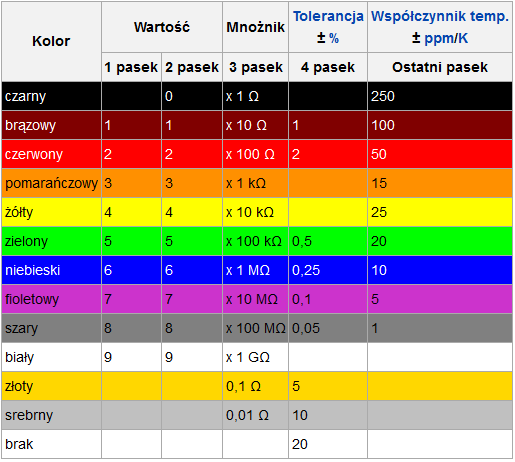
\includegraphics[scale=0.75]{oporniki}
\caption{Oznaczenia rezystorów}
\label{fig:oporniki}
\end{figure}
	
\begin{wrapfigure}{r}{0.5\textwidth}
\begin{center}
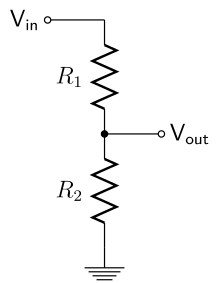
\includegraphics[width=0.48\textwidth]{v-divider}
\caption{Układ dzielnika napięcia}
\label{fig:divider}
\end{center}
\end{wrapfigure}

	Element ten jest kluczowy w celu ograniczenia przepływu prądu w obwodzie rękawicy, co pozwala na monitorowanie oporu wytwarzanego poprzez czujnik wygięcia. Sposób działania układu, nazywanego dzielnikiem napięcia jest pokazany na rysunku~\ref{fig:divider}, oraz wyraża się wzorem
	$$
		\nu_{out} = \nu_{in}\left[ \frac{R_2}{R_1+R_2}\right]
	$$
Wzór ten podaje napięcie wyjściowe $\nu_{out}$, które równa się napięciu wejściowemu $\nu_{in}$ przeskalowanemu przez stosunek rezystorów. W opisywanym przypadku jest to stosunek zastosowanego rezystora $4.7 k\Omega$ wyrażonego we wzorze poprzez $R_2$, do sumy tego rezystora wraz z oporem wytwarzanym poprzez czujnik wygięcia $R_1$ - który jak opisano w podrozdziale~\ref{subsec:wygiecie} jest zmienny. Oznacza to że im bardziej czujnik wygięcia jest zgięty, wytwarza on większy opór a co za tym idzie napięcie wyjściowe spada. Miara ta obrazuje jak bardzo palec jest zgięty i jest możliwa do uzyskania właśnie dzięki zastosowaniu układu dzielnika napięcia~\cite{v-divider}.


\section{Budowa rękawicy}
\label{sec:budowa}

W poniższej sekcji zaprezentowano sposób w jaki zostały złączone wszystkie elementy rękawicy wspomniane w sekcji~\ref{sec:przeglad}, aby była gotowa na oprogramowanie mikrokontrolera tworząc finałowy produkt. W tym celu została wybrana rękawica budowlana o grubych niciach ze ściągaczem wokół nadgarstka w celu zapewnienia komfortu, jak i precyzji położenia. Wybór ten również jest uzasadniony faktem początkowego planu dotyczącego wszycia materiału bezpośrednio w rękawice jak i elastyczności które zapewnia grubsza rękawica. Tak jak wspomniano w podsekcji~\ref{subsec:wygiecie}, do połączenia elementów została wykorzystana nić przewodząca. Dzięki grubym włóknom odstępu pomiędzy nićmi przewodzącymi prąd mogły być mniejsze, bez obawy przed spięciami w trakcie poruszania ręką. Dla tego projektu kontroler jest budowany dla lewej dłoni. Układ przewodów kontrolera jest zobrazowany na rysunku~\ref{fig:circuit}. Jest to jedynie obraz poglądowy, przedstawiony na płytce prototypowej a szczegółowy opis połączeń kontrolera zostanie opisany poniżej.

\begin{figure}[h]
\centering
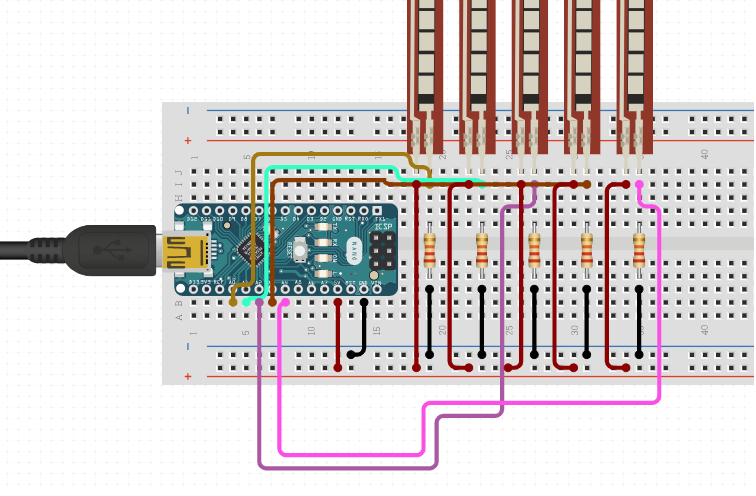
\includegraphics[width=\textwidth]{circuit}
\caption{Poglądowy układ kontrolera przedstawiający sposób podłączenia dzielnika napięcia}
\label{fig:circuit}
\end{figure}

Mikroprocesor został umieszczony na wysokości centralnej części dłoni, przy kciuku, skierowany złączem USB na zewnątrz, pozwalając na łatwe podłączenie przewodu zasilającego jak i również ustawienie wejść analogowych w stronę palców lewej dłoni. Z tej strony płytki Arduino będziemy też korzystać - zarówno przy wyprowadzaniu napięcia jak i uziemienia. Montaż samej płytki nie stanowi żadnego problemu ze względy na cztery otwory w rogach pozwalające na mocowanie, do którego została użyta zwykła nić do szycia. Aby stworzyć obwód wychodzący od pinu GND (z ang. Ground) czyli właśnie uziemienia, należy najpierw poprowadzić go przez rezystory. W tym celu wyjścia oporników zostały wygięte w pętle oraz zalutowane aby w łatwy sposób można było je przyszyć do rękawicy. Aby dodatkowo ułatwić sobie to zadanie - dodatkowo zostały one przyklejone bezpośrednio do materiału na bardzo małą ilość kleju. Umiejscowienie rezystorów jest po zewnętrznej wierzchniej stronie dłoni, zaczynając się na wysokości kontrolera, zmierzając szeregowo w stronę nadgarstka. W ten oto sposób nić przewodząca została poprowadzona na zewnętrzną część dłoni a następnie poprzez wszystkie pętle rezystorów, kończąc na ostatnim. Z drugiej strony rezystora dochodzi natomiast nić pochodząca z czujnika oporu. W tym celu podczas tworzenia czujników oporu pozostawiono 25 cm długości nici, co pozwoliło na przymocowanie sensorów, a następnie połączenie obwodu. Sensory zostały zaopatrzone w krótkie, 1-2 cm długości kawałki taśmy elastycznej która została przyklejona na czubku każdego z sensorów pozwalając na elastyczny ruch sensora bez zerwania nici. Taśma ta została przyszyta w czubkach palców co dało punkt zaczepu dla sensorów. W tym momencie pozwoliło to na wygodne używanie nici wychodzących z sensorów w celu zamknięcia obwodu. Z powodu dużego zagęszczenia nici, które nie mogą się ze sobą stykać podczas ruchu ręki, ważnym dla projektu było naprzemienne używanie przestrzeni na rękawicy od spodu jak i od góry. Dzięki temu nici uziemienia oraz napięcia mogą się krzyżować nie zaburzając przy tym odczytów z sensorów. W celu jak najlepszego zagospodarowania przestrzenią wokół sensorów, uziemienie kciuka oraz małego palca zostały umiejscowione na nicie wychodzącej z prawej strony sensora, natomiast napięcie po lewej stronie. Dla pozostałych palców ustawienie to jest odwrotne. Mając to na uwadze została poprowadzona nić od kciuka poprzez wyjście 3.3 V na płytce a następnie wzdłuż knykci rękawicy, pozwalając nicią odpowiedzialnym za napięcie w odpowiednich sensorach na przyczepienie się w celu poboru napięcia tworząc tym samym dodatnią stronę układu. Nici wychodzące z sensorów które natomiast nie zostały do tej pory użyte, zostały przeszyte poprzez wyjścia analogowe a następnie podłączone kolejno do odpowiadających im rezystorów. Wyjścia odpowiadające każdemu z palców zostały opisane w tabeli poniżej. 

\begin{center}
\begin{tabular}{|c|c|}
\hline
Palec & Wyjście analogowe \\ \hline
Kciuk & A3 \\ \hline
Wskazujący & A0 \\ \hline
Środkowy & A1 \\ \hline
Serdeczny & A6 \\ \hline
Mały & A7 \\ \hline
\hline
\end{tabular}
\end{center}

Sposób w jaki zostały dobrane wyjścia jest podyktowany zaleceniami o nie korzystaniu z wyjść analogowych A4 oraz A5 oraz pozostawieniu przestrzeni wokół wyjścia A3 przeznaczonego na kciuka, ponieważ jako jedyne połączenie musiało najpierw zmierzać w kierunku palców a następnie w dół w celu połączenia z rezystorem. Efekt końcowy pracy przedstawia zdjęcie~\ref{fig:glove}.

\improvement{Zmień zdjęcie rękawicy na lepsze i wpasuj je do rozdziału}
\begin{figure}[h]
\centering
%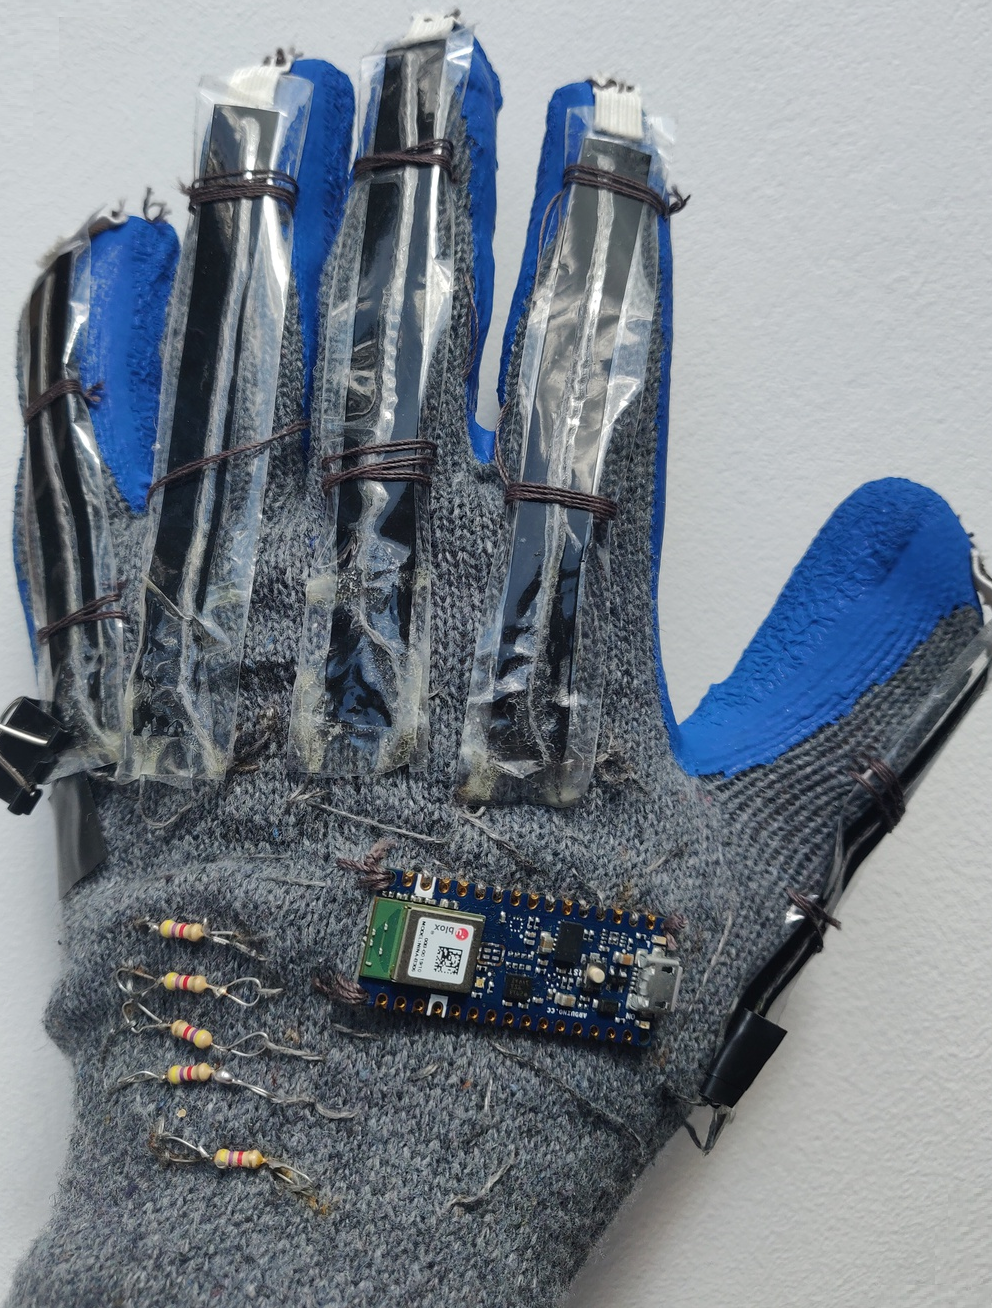
\includegraphics[width=\textwidth]{glove}
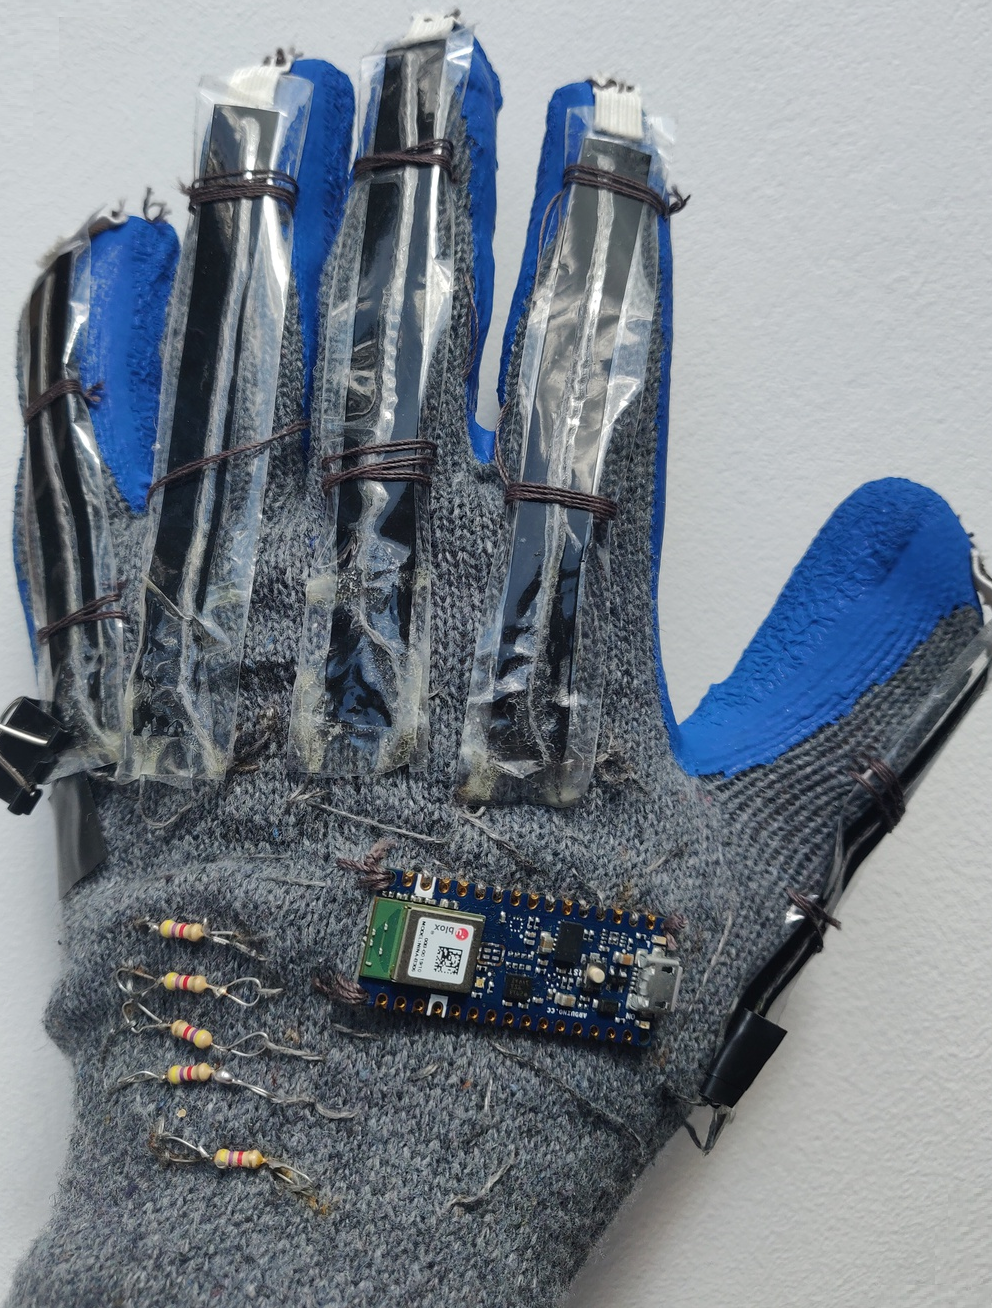
\includegraphics[scale = 0.2]{glove}
\caption{Efekt końcowy rękawicy-kontrolera}
\label{fig:glove}
\end{figure}

\section{Oprogramowanie mikrokontrolera}
\label{sec:oprogramowanie}


\section{Dalszy rozwój projektu}
\label{sec:rozwojPro}
